
\documentclass[a4paper,12pt]{article}
\usepackage[margin=2cm]{geometry}

% Pacchetti utili di base
\usepackage[utf8]{inputenc}   % codifica dei caratteri
\usepackage[T1]{fontenc}      % font encoding
\usepackage[italian]{babel}   % lingua italiana
\usepackage{graphicx}         % immagini
\usepackage{hyperref}         % link cliccabili
\usepackage{amssymb} % oppure amsfonts
\usepackage{float}
\usepackage{amsmath}

% Informazioni sul documento
\title{Reti di Calcolatori}
\author{Nicolò Giuliani}
\date{}


\begin{document}

\maketitle
\tableofcontents   % <-- genera automaticamente la pagina dell'indice
\newpage 

\section{Cosa è una rete di calcolatori?}
E' un insieme di calcolatori interconnessi tra loro per la comunicazione fra utenti, informazioni, risorse, ecc.
\subsection*{Classificazione}
\begin{itemize}
  \item Reti locali (LAN)
  \item Reti geografiche (WAN)
  \item Reti metropolitane (MAN)
\end{itemize}
Definiamo con \textbf{internet} la rete globale delle varie reti connesse tra loro via protocolli. \\
\subsection*{Prestazioni}
Misuriamo la velocità di una rete con i \textbf{bit} (b/s) o byte (B/s), ovvero gruppo da 8bit. Definiamo \textbf{ping} la latenza tra la partenza totale del pacchetto al suo arrivo dal destinatario, questo è data dalla tipologia di tecnologia utilizzata, protocolli e distanza fisica. Chiamiamo \textbf{jitter} la varianza media nel tempo di arrivo al destinatario dei pacchetti.
\begin{figure}[h] % [h] = qui (here)
    \centering
    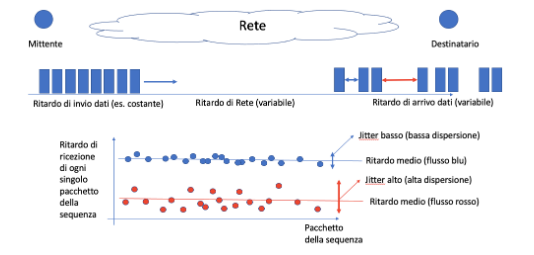
\includegraphics[width=0.7\textwidth]{img/jitter.png}
\end{figure}
\subsection*{Come ci si connette?}
Abbiamo bisogno di un insieme di componenti hardware e software:
\begin{itemize}
  \item \texttt{Scheda di rete}: trasmettere, codificare, decodificare i segnali elettrici in bit digitali.
  \item Driver: software che gestisce il dispositivo fisico con il S.O.
  \item Connettore (fisico) di rete: connettore standard della scheda di rete.
  \item \texttt{Mezzo di trasmissione}: fibre ottiche, cavi rame, ponti radio, ecc.
  \item \texttt{Protocolli}: regole via software per avere una piena combatibilità su tutti i dispositivi.
\end{itemize}
I vari calcolatori connessi in rete vengono divisi in \textit{host} e \textit{node}. Dividiamo in 2 macro categorie le infrastrutture di reti:
\begin{itemize}
  \item Peer to peer (P2P)
  \item Strutture a connessioni multiple, con cammino di segnali diretto o in sequenza.
\end{itemize}
\subsection*{Topologia}
Abbiamo come standard diverse schematiche di reti per connettere dei calcolatori:
\begin{itemize}
  \item a) Anello
  \item b) Stella
  \item c) Bus
  \item d) Albero
\end{itemize}
Ovviamente le reti più grandi utilizzano una struttura mista. 
\begin{figure}[h] % [h]
    \centering
    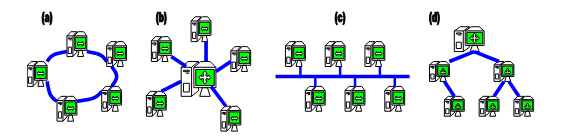
\includegraphics[width=0.7\textwidth]{img/topologia.png}
\end{figure} \\
\textit{Curisità}: In Italia abbiamo la rete \textbf{GARR} ovvero la rete italiana a banda ultralarga dedicata alla comunità dell'istruzione, della ricerca e della cultura.
\begin{figure}[h] % [h]
    \centering
    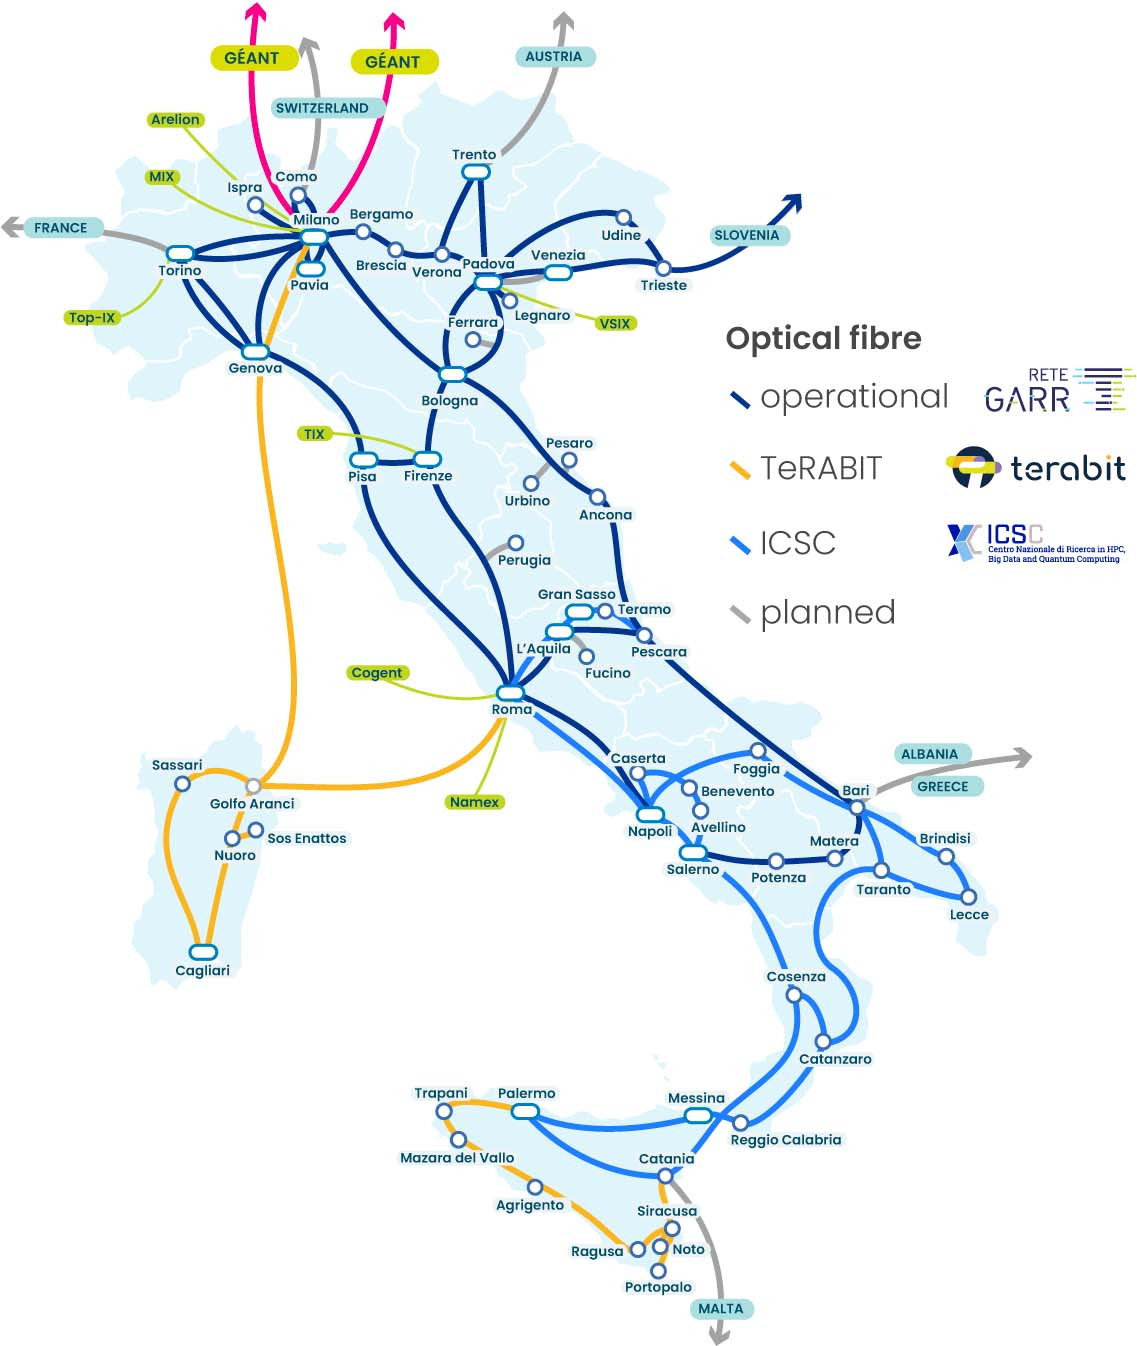
\includegraphics[width=0.35\textwidth]{img/garr.png}
    \caption{Mappa aggiornata a luglio 2024}
\end{figure} \\
\subsection*{Mezzo fisico di trasmissione}
Abbiamo 3 tipi di mezzo di trasmissioni:
\begin{itemize}
  \item Cavi / Fili metallici: segnali elettrici (corrente e variazione di tensione)
  \item Fibre ottiche: segnali luminosi dentro fibre di vetro
  \item Wireless: radiazioni elettromagnetiche nello spazio come onde radio e infrarossi
\end{itemize}
C'è anche una sostanziosa differenza tra hub e switch, nella topologia a stessa! L'hub (lavora in L1) "spara" il segnale elettrico in ogni porta e quindi capita più frequentemente collisione dei pacchetti (e la loro perdita). Costavano meno, e si "pregava" di più nel protocollo che sistemasse i pacchetti persi; andava bene per reti ridotte. Ad oggi gli switch che hanno preso la prevalenza nel mercato, anche a basso costo, ci permettono di minimizzare i conflitti reinstradando i pacchetti, lavora al L2 e basandosi sul MAC address del dispositivo connesso ad una porta reindirizza il pacchetto SOLO su quella porta. Mentre un router che lavora con indirizzi IP lavora ad L3.
\subsection*{Scheda di rete}
Componente del calcolatore che ha il connettore di rete e l'interfaccia tra scheda e mobo. Attraverso il proprio processore, memoria, chip, condensatori, ecc la scheda riceva/manda e codifica/decodifica i segnali elettrici/digitali. Il suo codice identificativo unico si chiama \textbf{MAC ADDRESS} (medium access control). \\
La scheda per comunicare con il calcolatore e il SO ha bisogno di un applicativo software che gestisca correttamente questa comunicazione, questo è il \textit{driver}.
\subsection{Canali di comunicazione}
Come abbiamo visto prima abbiamo P2P o canale broadcast. Soffermiamoci sul secondo, tutti i dispositivi comunicano nello stesso canale come siamo sicuri che non si trasmette/riceve nello stesso momento cordinando tutti? Attraverso l'indirizzo univoco del destinatario (MAC) e del mittente (MAC).
\begin{figure}[h] % [h]
    \centering
    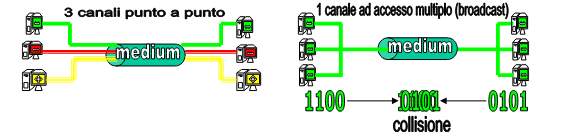
\includegraphics[width=0.7\textwidth]{img/p2p_broadcast.png}
\end{figure} \\
\subsection*{Tecnica di comunicazione}
\begin{itemize}
  \item \textbf{Commutazione a circuito} 
  Prima che due dispositivi inizino a comunicare viene stabilito il percorso (circuito dedicato) dalla sorgente al destinatario, per la durata della comunicazione il canale rimane riservato ed al termina viene liberato. Questo offre una buona velocità ma con alto ritardo e poco costante in caso di pause, tutto questo a costo per tempo. Un esempio è la rete telefonica.
  \item \textbf{Commutazione a pacchetto} 
  \texttt{Standard} per Internet e le comunicazioni broadcast. Tutti i dati vengono suddivisi in pacchetti indipendenti, spediti su canali diversi. Questo modello si può utilizzare sia per connessioni P2P che per le broadcast. Nel secondo caso dobbiamo definire anche: l'indirizzo del destinatario per ogni pacchetto, i pacchetti viaggiano tra flussi diversi di pacchetti. Questo offre una ottimizzazione delle risorse della rete con a costo però maggior ritardo nella comunicazione. Si paga per quantità di dati. 
\end{itemize}
Componendo in serie una sequenza di canali broadcast a commutazione di pacchetto, i nodi ricevitori devono di volta in volta
farsi carico di verificare se il pacchetto sia giunto a destinazione o, in caso contrario, possono provvedere all’inoltro del
pacchetto ricevuto sul successivo canale broadcast.
Il prezzo di questa tecnica è legato al maggiore ritardo per la comunicazione dei dati tra mittente e destinatario, dovuto
all’esigenza di iterare più volte la ricezione e l’inoltro di pacchetti su canali broadcast in sequenza.
Il vantaggio è legato al maggiore utilizzo dei canali ad accesso multiplo, e quindi alla possibilità di tariffare la comunicazione in
base ai dati trasmessi, e non in base al tempo necessario.
\begin{figure}[h]
    \centering
    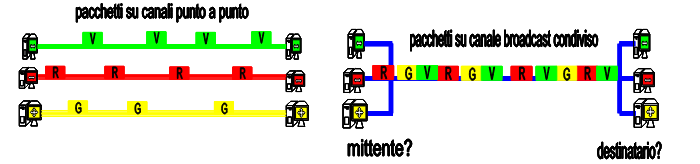
\includegraphics[width=0.6\textwidth]{img/commutazione.png}
\end{figure} \\
\subsection{Protocolli di rete organizzati a livelli}
Un protocollo è un insieme di regole e procedure di gestione dei processi di comunicazione. Quindi si è definito una \textit{archietettura} di rete divisa in livelli nel quale ognuno affronta problemi diversi, dal basso al alto si forniscono servizi. Questo insieme crea il protoccolo per l'interfaccia di rete. \\
Nel 1984 si è ufficializzato lo standard \textbf{ISO/OSI} (Open System Interconnection Reference Model), la struttura di rete è divisa in 7 livelli nel quale più ci troviamo in alto più più il modello di rete si semplifica.
\begin{figure}[h] % [h] = qui (here)
    \centering
    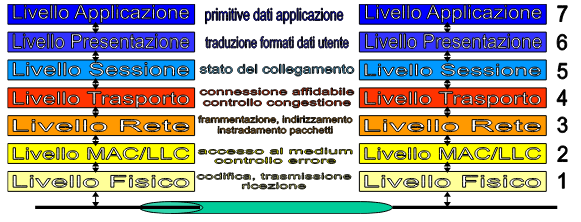
\includegraphics[width=0.9\textwidth]{img/iso-osi.png}
\end{figure} \\
L'architettura moderna di Internet utilizza solo 5 livelli del modello ISO/OSI, ogni livello riceve dati dai livelli superiori e li inserisce (incapsula) in “buste” con dati aggiuntivi, utili ad istruire il corrispondente livello del dispositivo ricevente.
\begin{itemize}
  \item Il livello trasporto imbusta i dati aggiungendo informazioni utili all’ordinamento e controllo della velocità di invio delle buste 
  \item Il livello rete frammenta i dati in pacchetti, decide il cammino sul quale inviare il pacchetto a seconda dell’indirizzo del destinatario
  \item I livello MAC/LLC esegue la consegna finale dei dati a dispositivi di una rete locale
\end{itemize}
.
\begin{figure}[h] % [h] = qui (here)
    \centering
    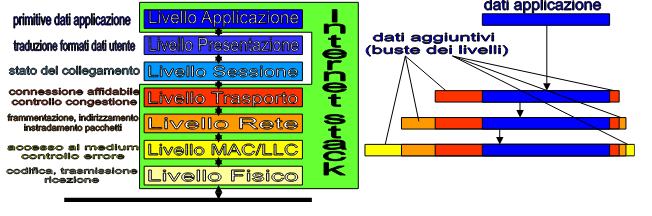
\includegraphics[width=0.9\textwidth]{img/internet.png}
\end{figure} \\
Vediamo ora nel dettaglio i 5 livelli del TCP/IP:
\begin{itemize}
  \item 1) livello fisico \\
  -  trasmissione sul canale di comunicazione fisicamente attraverso segnali analogici, derivanti da codifica dei segnali in bit. La velocità dei segnali analogici è pressochè quella cella luce, si misura però in bit/secondo + tempo di decodifica da analogico $\rightarrow$ digitale
  \item 2) livello MAC/LLC \\
  - rete locale (LAN). Frame.
  \item 3) livello rete \\
  - attraverso i router colleghiamo le LAN tra di loro, qui nasce internet. Pacchetti.
  \item 4) livello trasporto \\
  - garantire che i dati arrivino correttamente, in ordine e senza duplicati, tra due processi tra due macchine diverse (TCP/UDP).
  \item 5) livello applicazione \\
  - servizio in utilizzo, Dati (HTTP, FTP, SSH, $\dots$) 
\end{itemize}
Come si è sicuri che un frame sia arrivato a destinazione? Se ne occupa il LLC con il rilevamento degli errori, controllo del flusso e conferma di ricezione:
\begin{itemize}
  \item Si! il pacchetto arrivato a destinazione, il destinatario invia un frame di conferma (ACK)
  \item No! il mittente non ricevendo la conferma trasmette di nuovo il frame
\end{itemize}
\pagebreak
\section{Reti di reti e Internetworking}
Le reti locali sono connesse attraverso collegamenti organizzati in modo gerarchico, basati su calcolatori rappresentanti della rete locale (router) a loro volta collegati da linee dati veloci o dorsali (backbone).
\begin{center}
    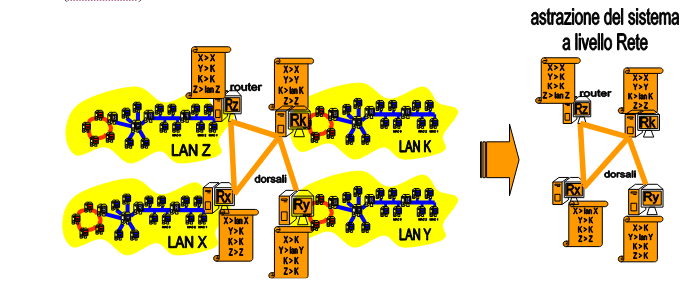
\includegraphics[width=0.6\textwidth]{img/Internetworking.png}
\end{center} 
\subsection{Internet protocol (IP)}
Il concetto di rete non si limita ora alla sola rete locale (LAN) ma si estende alla rete di reti globale (Internet).
\begin{itemize}
  \item Internet:
  \begin{itemize}
    \item nuovo tipo di indirizzamento globale e gerarchico (indirizzamento IP)
    \item instradamento dei pacchetti dal mittente al destinatario finale (forwarding)
    \item nuovi dispositivi amministratori del livello tre: router
    \item frammentazione dei dati da spedire in paccheti
    \item busta del pacchetto di livello rete con gli indirizzi di mittente e destinatario
  \end{itemize}
\end{itemize}
\subsection{Ipv4}
Un indirizzo IP viene associato a una e una sola interfaccia di rete (scheda di rete) che a sua volta ha una associazione univoca tra indirizzo MAC. \\
Vediamo le caratteristiche
\begin{center}
Ipv4 = 4byte (32bit) \\
xxx.xxx.xxx.xxx (da 0 a 255)
\end{center}
Indirizzo IP è sempre composto da due parti:
\begin{itemize}
  \item Numero della rete IP alla quale appartiene la scheda (\textbf{network number})
  \item Numero dell’interfaccia di rete (\textbf{host number}) all’interno della rete
\end{itemize}
Il valore dell’indirizzo IP determina la \textbf{classe} della rete: A,B,C (non si usano più).
\begin{center}
    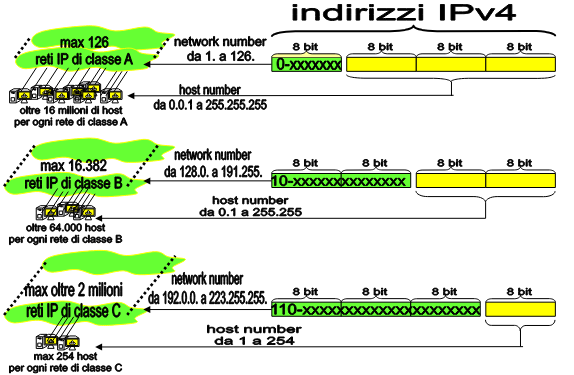
\includegraphics[width=0.6\textwidth]{img/classe.png}
\end{center} 
\subsection{Subnetwork}
Reti IP e router sono organizzati secondo una gerarchia, basata sul concetto di rete e sottorete.
\begin{itemize}
  \item indirizzo IP spezzato in due componenti logiche mediante maschera di rete (netmask)
  \begin{itemize}
    \item indirizzo di sottorete (subnetwork)
    \item host number dell’host appartenente alla sottorete
  \end{itemize}
\end{itemize}
\begin{center}
    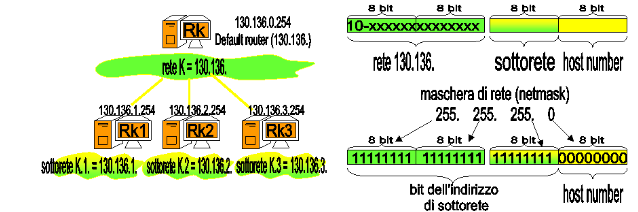
\includegraphics[width=0.8\textwidth]{img/inforete.png}
\end{center} 
Indirizzo IP, netmask e default router sono informazioni di configurazione del livello rete
\subsection{Forwarding}
Processo con cui un dispositivo di rete, come un router, riceve un pacchetto dati da una rete e lo invia verso un’altra rete, seguendo le informazioni contenute nell’header del pacchetto e nella tabella di routing del dispositivo.
\subsection{Routing}
Processo mediante il quale un dispositivo di rete, tipicamente un router, decide il percorso migliore che un pacchetto dati deve seguire per arrivare dalla sorgente alla destinazione. \\
\vspace{5px}\\
\textbf{Aggiornamento delle tabelle di forwarding dei router}: algoritmi di routing su Internet: Routing Information Protocol (RIP), Open Shortest Path First (OSPF), Border Gateway protocol (BGP).
\subsection{Protocollo ICMP}
Internet Control Message Protocol (ICMP); protocollo dei messaggi di controllo su Internet.
\begin{itemize}
  \item Standard per definire la comunicazione di informazioni utili alla gestione di Internet
  \item usato da host, router e gateway per scambiare informazioni di livello rete, usando pacchetti definiti con il protocollo IP
\end{itemize}
Vediamo delle applicazioni basate su ICMP
\begin{itemize}
  \item \textit{Ping}: test di verifica di connessione tra due host 
  \item \textit{Traceroute}: mostra la sequenza di router attraversati da un pacchetto per arrivare all’host destinazione
\end{itemize}
\subsection{ARP e RARP}
Quando un router riceve un pacchetto destinato a un indirizzo IP della propria sottorete, esso deve produrre un frame di livello MAC/LLC che riporti specificato l’indirizzo MAC del destinatario (e non l’indirizzo IP), per poterlo passare al livello MAC/LLC per la trasmissione sulla rete locale.
\begin{itemize}
  \item Address Resolution Protocol (ARP): 
  \begin{itemize}
    \item Usato se il router non conosce l’indirizzo MAC corrispondente all’indirizzo IP
    \item Il router genera un frame spedito a tutti i dispositivi della rete locale dove si chiede: “quale è l’indirizzo MAC del dispositivo che ha questo indirizzo IP”?
    \item Se tale dispositivo esiste, esso risponde con un frame di livello MAC indirizzato al router, nel quale viene evidenziato l’indirizzo MAC richiesto
  \end{itemize}
  \item Reverse-ARP (RARP):
  \begin{itemize}
    \item Domanda è “quale indirizzo IP corrisponde al dispositivo con questo indirizzo MAC”? (inverso di ARP)
  \end{itemize}
\end{itemize}
\begin{center}
    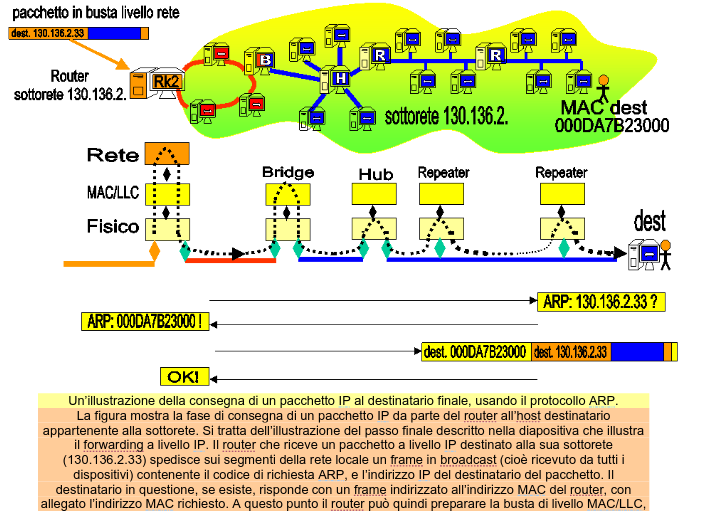
\includegraphics[width=0.6\textwidth]{img/arp.png}
\end{center} 
\subsection{DHCP}
\begin{itemize}
  \item Assegnazione dei numeri di rete di classe A, B, C
  \begin{itemize}
    \item vengono assegnati a enti, aziende ed organizzazioni che ne fanno richiesta, da parte di enti internazionali (RIPE, ICANN, ARIN, APNIC)
  \end{itemize}
  \item Assegnazione dei numeri di host ai dispositivi di una rete
  \begin{itemize}
    \item Assegnazione manuale
    \item Assegnazione automatica (\textbf{DHCP})
    \begin{itemize}
      \item Un server Dynamic Host Configuration Protocol si occupa dell/assegno dell’indirizzo IP agli host che ne fanno richiesta
      \item Un DHCP server dispone di un blocco di host number liberi per la sua rete
      \item DHCP server associa indirizzi IP a indirizzi MAC dei dispositivi che lo richiedono
      \item I dispositivi devono scegliere di affidarsi al server DHCP
    \end{itemize}
  \end{itemize}
\end{itemize}
\subsection{IPv6 e tunnelling IPv4}
Dal 1990 e' attivo IPv6, indirizzi estesi a 128 bit (16 Byte) (prima erano a 32bit). \\
\textbf{Tunneling}: spedire pacchetti IPv6 in buste IPv4.
\subsection{Livello trasporto: TCP / UDP}
I protocolli di Internet di quarto livello (trasporto) sono essenzialmente il Transmission Control Protocol (TCP) e lo User Data Protocol (UDP).
\begin{itemize}
  \item Servizio trasporto affidabile (protocollo \textbf{TCP}): servizio di tipo connection-oriented
  \begin{itemize}
    \item numero di porta del socket TCP
    \item eliminazione dei pacchetti duplicati
    \item Pacchetti conferma della ricezione (acknowledgment di livello trasporto) + Pacchetti non ricevuti (non confermati entro timeout) spediti di nuovo
  \end{itemize}
  \item  Servizio trasporto non affidabile (protocollo \textbf{UDP}): servizio connectionless 
\end{itemize}
\begin{center}
    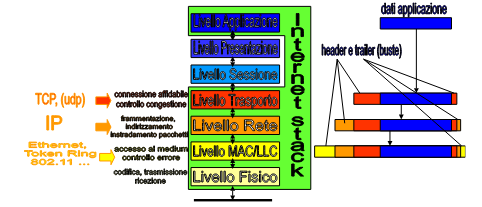
\includegraphics[width=0.6\textwidth]{img/tcp.png}
\end{center} 
\subsection*{TCP}
E' il protocollo di livello trasporto usato di fatto su Internet (TCP/IP).
\begin{itemize}
  \item Socket (indirizzo ip + porta del livello superiore)
  \item applicazioni in attesa sul socket
  \item client invia richiesta TCP al socket server
  \item server risponde "ok" (se il socket del server esiste e non e' occupato) 
  \item il client (se riceve "ok") puo' inziare a inviare i dati di configurazione TCP
  \item ora avviene il vero scambio a livello TCP
  \item rilascio della connessione (si liberano le porte)
\end{itemize}
\begin{center}
    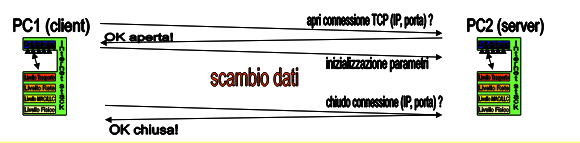
\includegraphics[width=0.8\textwidth]{img/porte.png}
\end{center} 
\subsection{Controllo di flusso e congestione}
Problema: la latenza di rete (tempo di andata e ritorno dei pacchetti) è alta
\begin{itemize}
  \item Invio pacchetto e attendo conferma prima di inviare il successivo?
  \begin{itemize}
    \item Solo un pacchetto in tutto il cammino: troppo lento!!!
  \end{itemize}
  \item  Invio tutti i pacchetti uno di seguito all’altro in un colpo solo?
  \begin{itemize}
    \item Possibile congestione nei router intermedi, che perdono pacchetti: troppo veloce!
    \item Possibile saturazione del destinatario, che riceve pacchetti troppo velocemente!
  \end{itemize}
\end{itemize}
\begin{itemize}
  \item  Scopo del \textbf{controllo di flusso}: inviare pacchetti al massimo ritmo sostenibile dal destinatario finale
  \item Scopo del \textbf{controllo di congestione}: inviare pacchetti al massimo ritmo sostenibile dal router più lento della rete dal mittente al destinatario finale
\end{itemize}
 Esistono vari metodi: meccanismo a \textbf{finestra scorrevole} (sliding window, SW).
 \begin{center}
    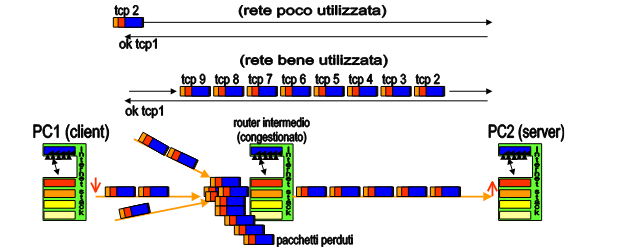
\includegraphics[width=0.8\textwidth]{img/congestione.png}
\end{center} 
Una finestra scorrevole (sliding window, SW) è un valore intero, (es. $n \in \mathbb{N}$) e rappresenta il numero massimo di pacchetti che un mittente può spedire di seguito, in attesa di ricevere la loro conferma.
\begin{itemize}
  \item Ogni mittente TCP spedisce al massimo ritmo possibile un gruppo di SW pacchetti
  \item \textbf{Controllo di flusso}: non spedisce più di SW pacchetti oltre l’ultimo non confermato
  \item \textbf{Controllo della congestione}: spedisce un numero SW variabile di pacchetti
  \begin{itemize}
    \item Se SW pacchetti spediti sono tutti confermati, aumenta SW ($2 \to 4 \to 8 \to \dots$)
    \item Appena un pacchetto degli SW inviati non viene confermato (scade il timeout)
    \begin{itemize}
      \item Assume che ciò sia dovuto a congestione su un router
      \item Riparte da SW minimo
    \end{itemize}
    \item Cerca di accelerare il ritmo gradualmente e, appena scopre la congestione, rallenta.
  \end{itemize}
\end{itemize}
 \begin{center}
  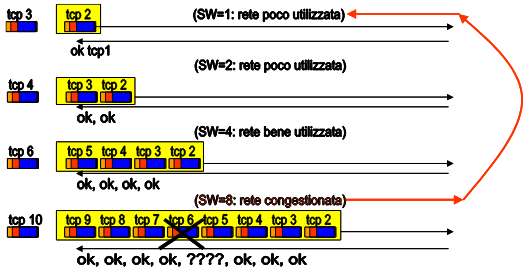
\includegraphics[width=0.6\textwidth]{img/congestione2.png}
\end{center} 
\subsection*{TCP/IP}
Cosa serve per configurare un host per la connessione a Internet?
\begin{itemize}
  \item Installare il dispositivo o scheda di rete
  \begin{itemize}
    \item Creare istanza dello stack TCP/IP e PPP per il dispositivo (modem)
    \item (Installare firewall per impedire accessi esterni all’host?)
    \begin{itemize}
      \item Bloccare l’accesso ai dati e alle applicazioni degli intrusi
      \begin{itemize}
        \item Filtrare i pacchetti a livello rete
        \item Firewall: è il primo router visto dall’esterno della rete, che filtra i pacchetti
      \end{itemize}
    \end{itemize}
  \end{itemize}
  \item Informazioni da fornire (manualmente, o attraverso DHCP server dell’ISP)
\end{itemize}
 \begin{center}
  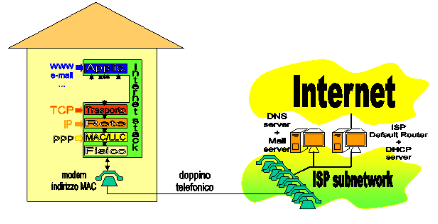
\includegraphics[width=0.6\textwidth]{img/isp.png}
\end{center} 
\subsection{DNS e nomi di dominio}
Gli utenti preferiscono usare nomi per le risorse in rete, anziché indirizzi IP. \\
\textit{Problema}: I protocolli di rete e i router pretendono di usare indirizzi IP. 
\begin{itemize}
  \item Domain Name System (DNS)
  \begin{itemize}
    \item Basato su una catena di server DNS organizzati gerarchicamente
    \begin{itemize}
      \item Ogni host in rete deve conoscere almeno un DNS server
      \item Ogni server DNS conosce almeno un DNS server superiore
    \end{itemize}
    \item I server ricevono richieste (protocollo DNS) e forniscono indirizzi IP 
    \item Se un server non conosce la risposta inoltra la richiesta DNS a un server superiore
    \item I server DNS radice (DNS root server) conoscono tutti i domini e i loro IP! (ma sono pochi e costosi)
  \end{itemize}
\end{itemize}
 \begin{center}
    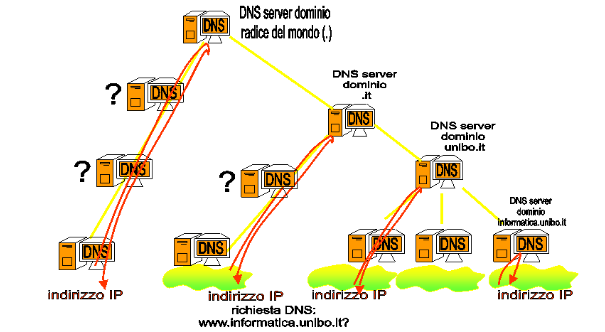
\includegraphics[width=0.6\textwidth]{img/unibo.png}
\end{center} 
\subsection{Livello applicazione}
l livello applicazione (si appoggia sul livello trasporto (in particolare sul protocollo TCP)): primitive e protocolli per spedire e ricevere dati delle applicazioni.
\begin{itemize}
  \item Posta elettronica (SMTP, POP3, IMAP)
  \item World Wide Web (HTTP)
  \item DNS: Domain Name Service (protocollo DNS)
\end{itemize}
 \begin{center}
    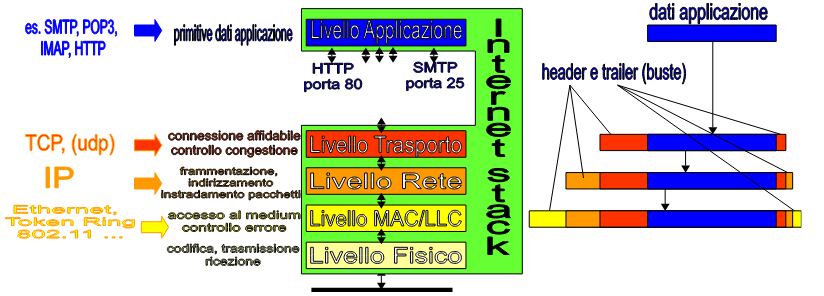
\includegraphics[width=1\textwidth]{img/completo.png}
\end{center} 
\subsection*{Servizi Client/Server e Peer to Peer}
Le applicazioni e i servizi su Internet possono essere realizzati secondo due modalità architetturali
\begin{itemize}
  \item \textbf{Architettura Client/Server}
  \item \textbf{Architettura Peer to Peer (P2P)}
  \item Servizi ibridi
\end{itemize}
\subsection{Servizi differenziati e Internet2}
Un aspetto critico della comunicazione su Internet è la mancanza di garanzie sui tempi di consegna dei dati (qualità del servizio).
\begin{itemize}
  \item Posso imporre che i pacchetti arrivino tutti (servizio connection-oriented di TCP)
  \item Non posso imporre che i pacchetti arrivino entro tempi fissati su Internet
  \begin{itemize}
    \item Tutti i pacchetti sono distribuiti con la stessa urgenza
  \end{itemize}
  \item \textbf{Internet2}
  \begin{itemize}
    \item Nuove linee dorsali e nuovi router
    \item I router spediscono prima i pacchetti urgenti, e poi quelli non urgenti
    \item Riservare le risorse lungo il cammino per comunicare i dati
    \item Garantisce la qualità del servizio su tutto il collegamento mittente-destinatario
  \end{itemize}
\end{itemize}
\section{Sicurezza di rete}
Alla base troviamo la criptografia con chiave condivisa su testo attraverso algoritmo in chiaro.
\begin{figure}[H]
    \centering
    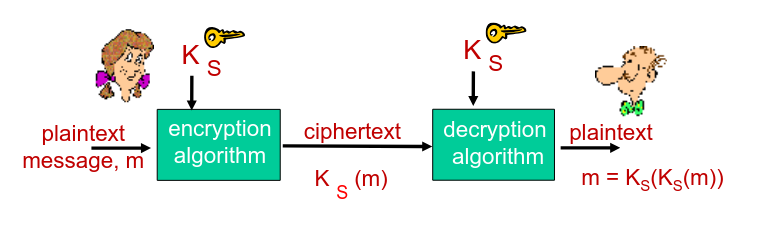
\includegraphics[width=0.7\textwidth]{img/chiave.png}
\end{figure}
Come ci mettiamo d'accordo sulla chiave comune?
\begin{itemize}
  \item Substitution cipher: sostituiamo una lettera dell'alfabeto con un'altra.\\
  $\to$ \textit{Encryption key:} mappiamo 26 lettere con altre 26 lettere.
  \item $n$-substitution ciphers: cicliamo $n$ cifrai ad ogni lettera.\\
  $\to$ \textit{Encryption key:} ciclare $n$-cifrai di 26 lettere.
  \item DES (Data Encryption Standard): input text di 64bit, chiave di 56bit. 16 round di funzione su 48bit della chiave. 
  \label{sec:des}
  \begin{figure}[H]
    \centering
    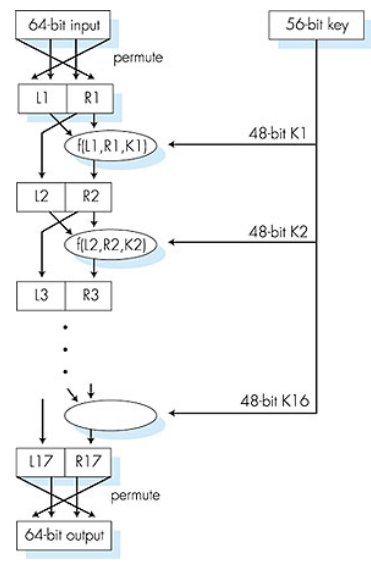
\includegraphics[width=0.3\textwidth]{img/des.png}
\end{figure}
  \item AES (Advanced Encryption Standard): rimpiazzo del DES, chiave da 128/192/256 bit, 10/12/14 round.
\end{itemize}
Abbiamo detto che nella \textbf{symmetric key crypto} il sender e receiver devono condividere la chiave segreta. Ma non è possibile avere una chiave senza una comunicazione insicura precedentemente. Come risolviamo?
\paragraph{Public key crypto} Non abbiamo sender e receiver con una chiave condivisa, ma
\begin{itemize}
  \item \textit{public encryption key}: condivisa a tutti $K_B^{-}$
  \item \textit{private decryption key}: solo receiver $K_B^{+}$
  \begin{align*}
    \text{msg} = K_B^{-}(K_B^{+})
  \end{align*}
\end{itemize}
  \begin{figure}[H]
    \centering
    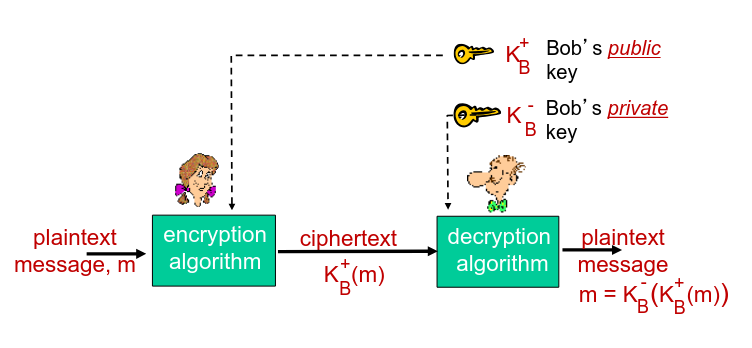
\includegraphics[width=0.7\textwidth]{img/public.png}
\end{figure}
\subsection{RSA}
\label{sec:rsa}
Così abbiamo ottenuto \textit{RSA} (Rivest, Shamir, Adelson algorithm). Come lo implementiamo?
\begin{itemize}
  \item $e$ chiave pubblica
  \item $d$ chiave privata
  \item $n$ prodotto di numeri primi
\end{itemize}
Sapendo che nella aritmetica modulare possiamo fare
\begin{align*}
  (a \bmod n)^d \bmod n = a^d \bmod n
\end{align*}
Quindi per cifrare facciamo
\begin{align*}
  c = m^e \bmod n
\end{align*}
e per decifrare
\begin{align*}
  c^d \bmod n = m
\end{align*}
e otteniamo
\begin{align*}
  \bigl(\underbrace{m^e \bmod n}_{c}\bigr)^d \bmod n \\
  m^{ed} \bmod n \\
  \to \boxed{m \equiv_n m^{ed}}
\end{align*}
Come scegliamo le chiavi?
\begin{itemize}
  \item Presi $p$ e $q$ primi da 1024bit
  \item Calcoliamo $n=pq, \, z=(p-1)(q-1)$
  \item Scegliamo $e \, (<n)$ tale che $mcd(e,z)=1$
  \item Scegliamo $d$ tale che $ed \equiv_z 1$ (ovvero $ed-1$ sia divisibile per $z$) \\
  $\to$ Abbiamo ora chiave pubblica $K_B^+ = (n,e)$ e chiave privata $K_B^- = (n,d)$ 
\end{itemize}
Possiamo anche notare la proprietà
\begin{align*}
  K_B^{-}(K_B^{+}) = m = K_B^{+}(K_B^{-})
\end{align*}
Vediamo quanto è sicuro la RSA. Supponiamo di conoscere la chiave pubblica $(n,e)$ dobbiamo trovare ora la chiave privata $(n,d)$. Quanto è difficile trovare $d$?
\begin{align*}
  d \equiv_{(p-1)(q-1)} e^{-1}
\end{align*}
Quindi dobbiamo trovare $p$ e $q$ partendo da $n=pq$. Qui dovremmo risolvere dei problemi di fattorizzazione su numeri grandi numeri (1024bit / 617 cifre decimali). Il costo computazionale richiederebbe migliardi di anni.\\
\vspace{1px}\\
Nella realtà calcolare RSA ad ogni connessione sarebbe computazionale costosto (per colpa del calcolo delle potenze), quindi facciamo RSA per condividere una chiave comune. Poi facciamo connessione a chiave simmetrica.
\subsection{Autenticazione}
Come proviamo la nostra identità tra client e server?
\begin{itemize}
  \item ap 1.0: Io sono $x$
  \item ap 2.0: IP + Io sono $x$
  \item ap 3.0: IP + password + Io sono $x$
  \item ap 3.1: IP + encrypted password + Io sono $x$
  \item ap 4.0: scegliamo numero \textbf{nonce} (\textit{once-in-a-lifetime}) $R$, client dice "Io sono $x$", il server manda $R$ al client, il client risponde con $K(R)$ criptato con chiave comune. Il problema è che serve chiave condivisa
  \label{sec:nonce}
  \begin{figure}[H]
    \centering
    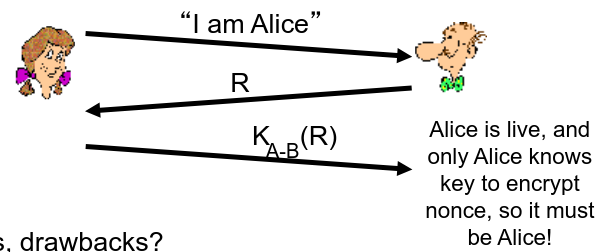
\includegraphics[width=0.6\textwidth]{img/ap4.png}
\end{figure}
  \item ap 5.0: Io sono $x$, server manda once $R$, il client risponde con la criptazione su chiave privata $K_A^{-} (R)$, il server chiede di mandargli la chiave pubblica $K_A^{+}$ e controlla se $R = K_A^{+}(K_A^{-} (R))$.
  \begin{figure}[H]
    \centering
    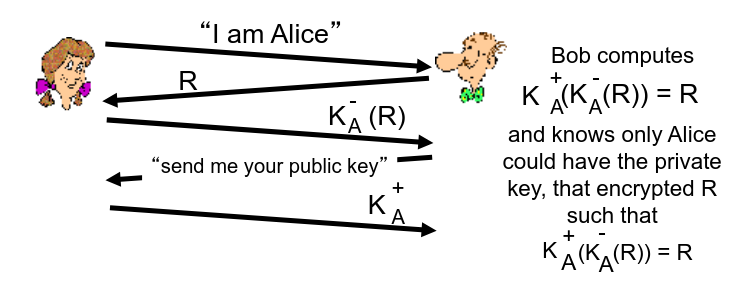
\includegraphics[width=0.7\textwidth]{img/ap5.png}
\end{figure}
\textit{Security hole}: l'attaccante posa come server al client e come client al server.
\end{itemize}
\subsubsection{Digital signatures}
Il sender spedisce il messaggio $m$ criptandolo con la sua chiave privata $K_B^{-}$ creato il messaggio firmato $K_B^{-}(m)$. Così il ricevente capisce se lo ha mandato il client facendo $K_B^{+}(K_B^{-}(m))=m$. \\
\textit{Il problema?} Fare public-key-encrypt su lunghi messaggi è computazionalmente costoso.\\
\begin{itemize}
  \item Hash function: applichiamo $H$ su $m$ e otteniamo il messaggio di lunghezza fissa $H(m)$. Poi dopo applichiamo la criptazione.\\
  $\to$ \textbf{Digital signature}: hashare un messaggio e poi criptarlo/decriptarlo su chiave privata e pubblica.
\end{itemize}
Soffre sempre di man in the middle (ap 5.0).
\subsubsection{Certification authority}
Una entità $E$ (persona, router, ecc) registra la sua chiave pubblica con CA, $E$ prova la sua identità al CA, CA collega $E$ alla sua chiave pubblica.
  \begin{figure}[H]
    \centering
    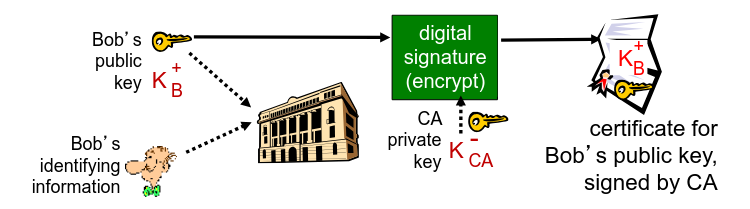
\includegraphics[width=0.7\textwidth]{img/cert.png}
\end{figure}
Il ricevente come ottiene la chiave pubblica del mandante? Ottiene il certificato dal client e si applica la chiave pubblica del CA sul certificato
  \begin{figure}[H]
    \centering
    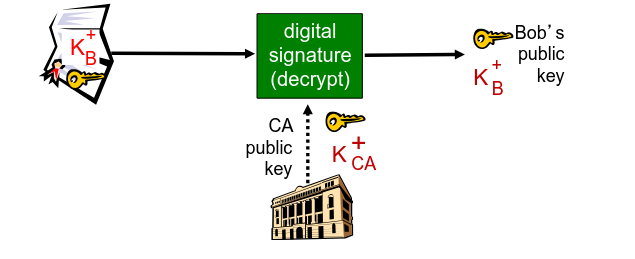
\includegraphics[width=0.5\textwidth]{img/cert2.png}
\end{figure}
Ovvero facciamo $K_B^{+} = K_{CA}^{-}(K_{CA}^{+}(K_B^{+})$ cosi mandiamo in modo sicuro la chiave pubblica del client. (Es. TLS per HTTPS)
\subsection{Securing e-mail}
Come mandiamo una mail $m$ sicura?
\begin{itemize}
  \item Chiave simmetrica casuale $K_S$
  \item Spediamo il messaggio criptato $K_S(m)$ e la chiave pubblica criptata $K_S(K_B^+)$
  \item Per decriptarlo si utilizza la chiave privata per ottenere $K_S$
  \item Utilizziamo $K_S$ per decriptare $m$
\end{itemize}
  \begin{figure}[H]
    \centering
    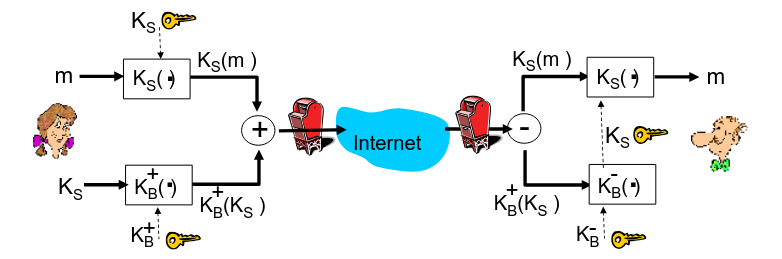
\includegraphics[width=0.7\textwidth]{img/mail.png}
\end{figure}
\begin{align*}
  K_B^-(K_B^+(K_S)) = K_S
\end{align*}
\paragraph{Autenticazione online (non sicura)}
Spediamo il messaggio con Hash condiviso $H(m)$ + criptazione su chiave pubblica/privata.
  \begin{figure}[H]
    \centering
    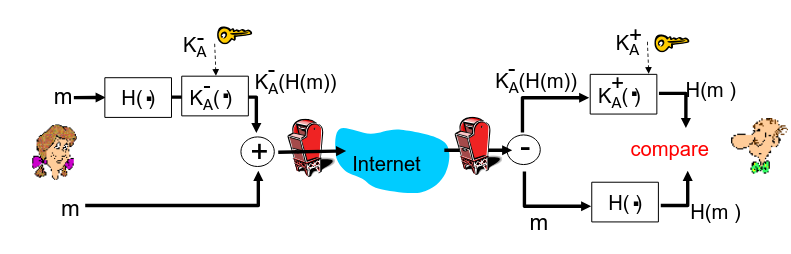
\includegraphics[width=0.7\textwidth]{img/nonsicuro.png}
\end{figure}
\paragraph{Autenticazione online (sicura)}
\label{sec:auth_sicura}
Spediamo messaggio su hash comune $H(m)$, criptato su chiave privata sender + chiave simmetrica $K_S$ su chiave pubblica receiver $K_S(K_B^+)$.
  \begin{figure}[H]
    \centering
    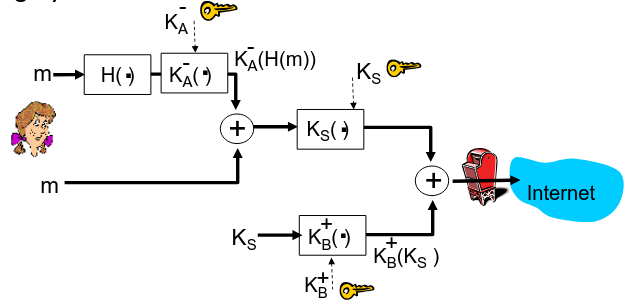
\includegraphics[width=0.6\textwidth]{img/sicuro.png}
\end{figure}
\begin{align*}
  K_B^-(K_B^+(K_S)) = K_S \\
  K_S(K_A^-(H(m)) + m) = K_A^-(H(m)) + m \\
  K_A^+(H(m)) = H(m) \text{ da confrontare con la nostra $H$ t.c.} =H(m) \\
\end{align*}
Il receiver deve conoscere la sua chiave privata, la chiave pubblica del sender e la hash function che è pubblica.
\subsection{Securing TCP connections: SSL}
  \begin{figure}[H]
    \centering
    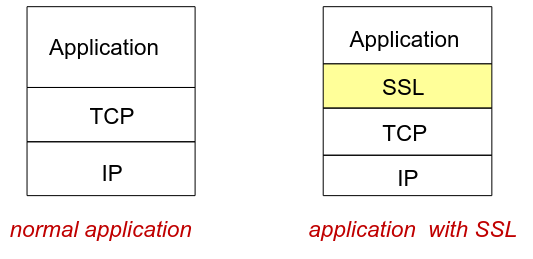
\includegraphics[width=0.4\textwidth]{img/ssl.png}
\end{figure}
SSL offre una API alle applicazioni (nella maggior parte dei LP).\\
Potremmo fare qualcosa come per \hyperref[sec:auth_sicura]{autenticazione online (sicura)} ma ci serve uno stream di dati costante.\\
Attraverso un \textbf{handshake} possiamo autenticare il sender e receiver.
  \begin{figure}[H]
    \centering
    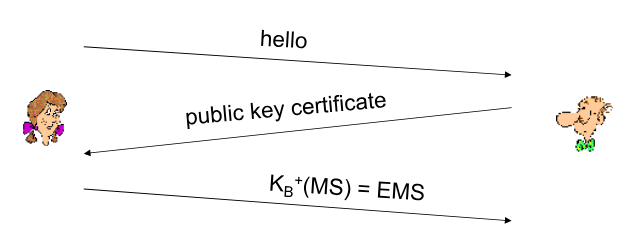
\includegraphics[width=0.6\textwidth]{img/toy.png}
\end{figure}
\begin{itemize}
  \item MS: master sicret
  \item EMS: encrypted master sicret
\end{itemize}
Ovviamente è cattiva pratica utilizzare la stessa chiave per più di 1 operazione di criptazione, si utilizzano diverse chiavi \textbf{MAC} (message authentication code)
\begin{itemize}
  \item $K_C$: chiave di criptazione client to server
  \item $M_C$: chiave MAC client to server
  \item $K_S$: chiave di criptazione server to client
  \item $M_S$: chiave MAC server to client
\end{itemize}
Via TCP come suddividiamo il pacchetto fra data e MAC?
  \begin{figure}[H]
    \centering
    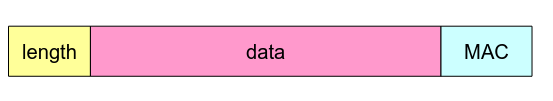
\includegraphics[width=0.6\textwidth]{img/MAC.png}
\end{figure}
Come rendiamo sicuro il MAC in modo che se qualcuno lo sniffi non lo posso riutilizzare?
\begin{align*}
  MAC = <type, \, sequence, \, data>
\end{align*}
con $type$ che indica la tipologia di pacchetto (mess, handshake, chiusa conn., ecc)
  \begin{figure}[H]
    \centering
    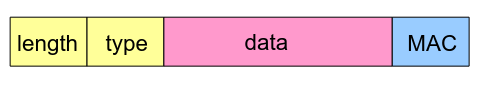
\includegraphics[width=0.5\textwidth]{img/type.png}
\end{figure}
  \begin{figure}[H]
    \centering
    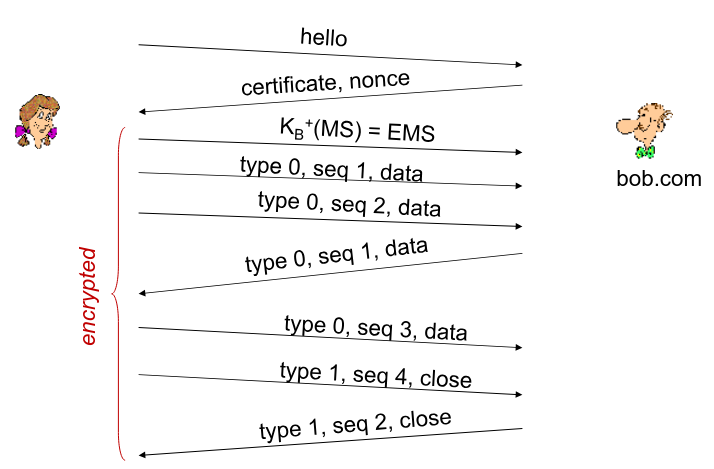
\includegraphics[width=0.5\textwidth]{img/toysec.png}
\end{figure}
Questo modello di SSL semplificato non basta, tipo se volessimo cambiare protocollo di criptazione? Specificare il protocollo scelto, ecc?
\paragraph{Comuni modelli di SSL simmetrici cifrai} 
\begin{itemize}
  \item \hyperref[sec:des]{DES}
  \item 3DES
  \item RC2
  \item RC4
\end{itemize}
\paragraph{Comuni modelli di SSL su chiave pubblica/privata}
\begin{itemize}
  \item \hyperref[sec:rsa]{RSA}
\end{itemize}
\subsubsection{Real SSL}
Attraverso l'\textbf{handshake} possiamo fare autenticazione server, negoziazione su scelta del algoritmo di criptazione, stabilire le chiavi e opzionalmente autenticazione client.
\begin{itemize}
  \item client manda la lista di algoritmi di criptazione supportati
  \item il server risponde: choice algoritmo + certificato + server \hyperref[sec:nonce]{nonce}
  \item client controlla il certificato, estraee chiave pubblica server, genera pre\_master\_secret, la cripta con chiave pubblica server e glielo spedisce
  \item client e server indipententemente calcolano decriptazione e MAC key dalle pre\_master\_secret e nonce
  \item client manda MAC di tutti gli handshake 
  \item server manda MAC di tutti gli handshake 
\end{itemize}  
Protocollo:
  \begin{figure}[H]
    \centering
    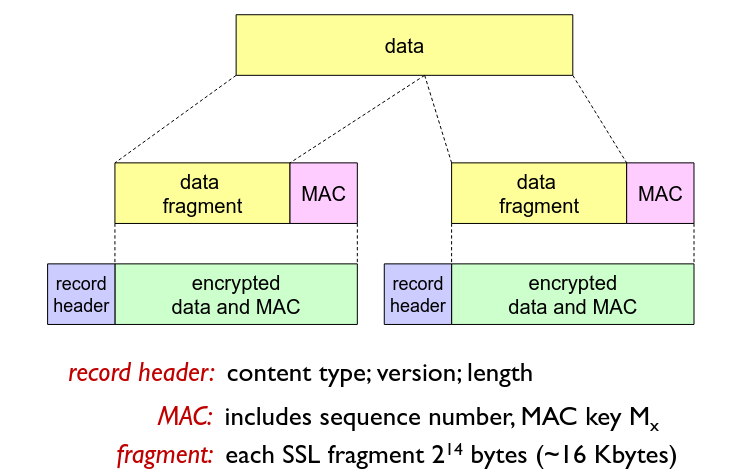
\includegraphics[width=0.5\textwidth]{img/sslreal.png}
\end{figure}
Formato del pacchetto:
  \begin{figure}[H]
    \centering
    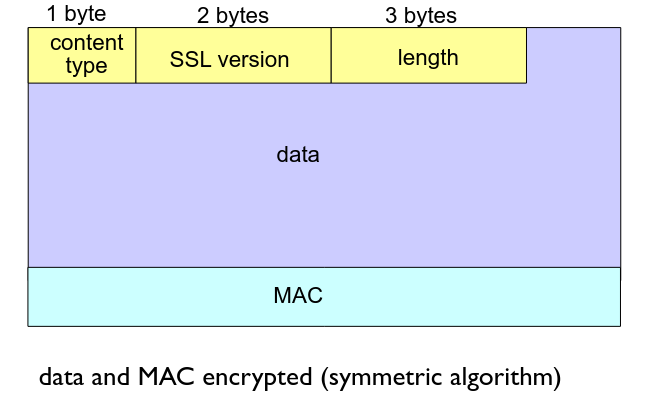
\includegraphics[width=0.5\textwidth]{img/formatoreal.png}
\end{figure}
Connessione:
  \begin{figure}[H]
    \centering
    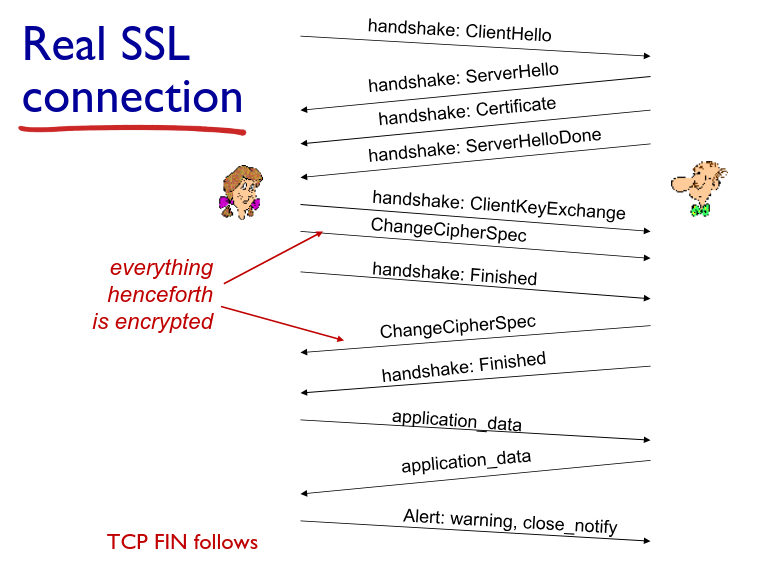
\includegraphics[width=0.7\textwidth]{img/connessionereal.png}
\end{figure}
\subsection{Network layer security: IPsec}
Come rendiamo sicura la trasmissione tra due reti?
\subsubsection{VPN}
Criptiamo prima di andare in internet pubblico, attraverso la logica separata dal resto del traffico.\\
Il sender e reciver sono pubblici (header) mentre il traffico diventa criptato.\\
\vspace{1em}\\
Alla base delle VPN troviamo \textbf{IPsec} ovvero un insieme di protocolli per proteggere comunicazioni su rete IP cifraindo i dati che viaggiano tra due dispositivi.
\begin{itemize}
  \item Confidenzialità (dati cifrati)
  \item Integrità (dati non possono essere modificati senza accorgersene)
  \item Autenticazione (di chi sta parlando)
  \item Anti-replay (impedisce il riutilizzo dei pacchetti in attacchi)
\end{itemize}
Per implementarlo abbiamo due opzioni:
\begin{itemize}
  \item \textbf{AH} (Authentication Header): Garantisce autenticazione e integrità, non cifra i dati e non garantisce confidalietà
  \item \textbf{ESP} (Encapsulating Security Payload): Garantisce cifratura + autenticazione + confidalietà
\end{itemize}
Modalità di funzionamento (Ipsec lavora a livello rete)
\begin{itemize}
  \item \textbf{Transport Mode}: i client si occupano del IPsec 
  \begin{figure}[H]
    \centering
    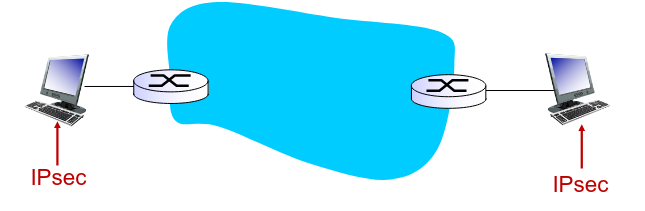
\includegraphics[width=0.7\textwidth]{img/transport.png}
\end{figure}
  \item \textbf{Tunneling Mode}: i router si occupano del IPsec 
    \begin{figure}[H]
    \centering
    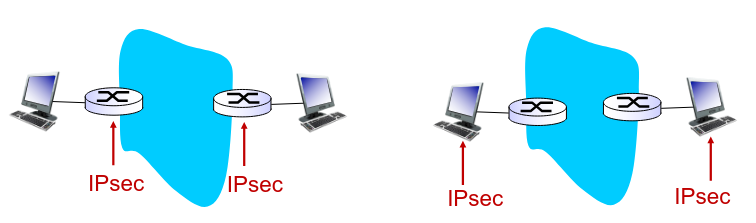
\includegraphics[width=0.7\textwidth]{img/tunnelling.png}
\end{figure}
\end{itemize}
    \begin{figure}[H]
    \centering
    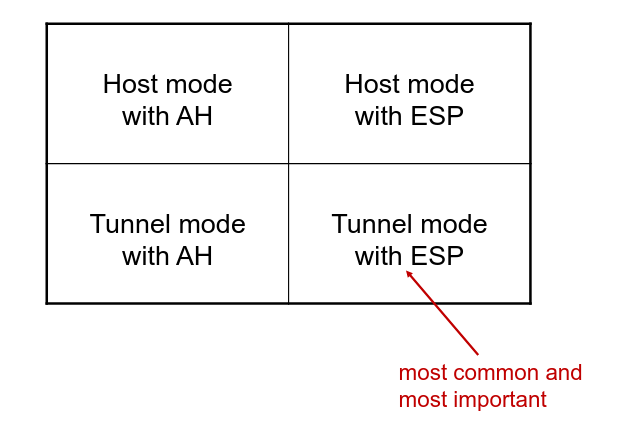
\includegraphics[width=0.7\textwidth]{img/common.png}
\end{figure}
\paragraph{Security associations (SAs)} Prima di iniziare a spedire i dati dobbiamo fare "security associations" fra sender e receiver. Una SA è l’insieme di parametri che stabiliscono algoritmi, chiavi e regole per cifrare/autenticare i pacchetti.
    \begin{figure}[H]
    \centering
    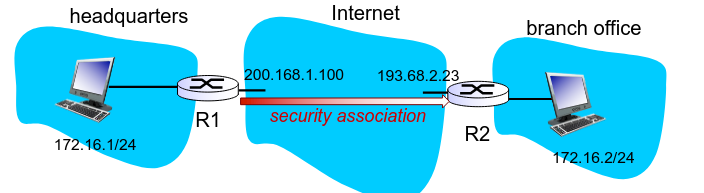
\includegraphics[width=0.7\textwidth]{img/sas.png}
\end{figure}
\paragraph{Security Association Database (SAD)} Il Security Association Database (SAD) è la struttura dati in cui un sistema che usa IPsec salva tutte le Security Associations (SA) attive.
    \begin{figure}[H]
    \centering
    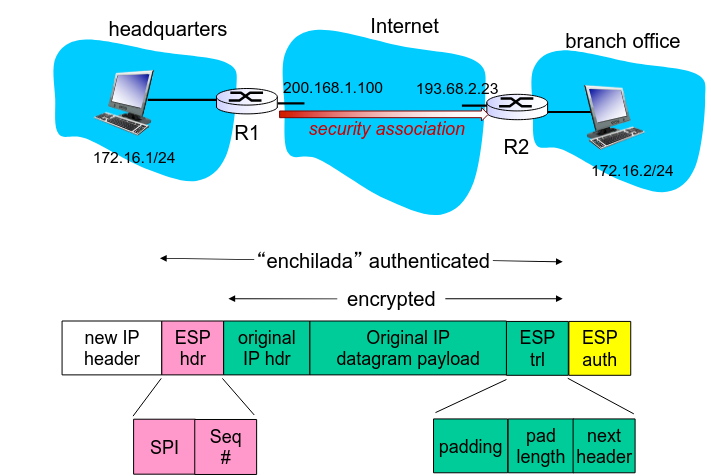
\includegraphics[width=0.7\textwidth]{img/sad.png}
\end{figure}
\begin{itemize}
  \item ESP trailer: bit padding per arrivare a una certa dimensione
  \item ESP header:
  \begin{itemize}
    \item SPI, so receiving entity knows what to do
    \item Sequence number, to thwart replay attacks
  \end{itemize}
  \item MAC in ESP auth field is created with shared secret key
\end{itemize}
\paragraph{Security Policy Database (SPD)} Il Security Policy Database (SPD) è la struttura dati che contiene le regole di sicurezza che stabiliscono quale traffico IP deve essere protetto e come.
SPD indica cosa se e come proteggere un pacchetto, SAD indica come farlo (chiavi e parametri). 
\subsection{Securing wireless LANs}
\textbf{WEP}: stabilire rete temporanea tra due dispositivi wifi. Molto efficiente da implementare via hw o sfw.\\
Sicuro come modello matematico (criptazione 802.11), non sicuro perchè durante la security association l'header dei pacchetti (criptato con la stess achiave WEP) è noto e quindi per analisi di correlazione tra i pacchetti si riesce a fare bruteforce per decriptare i pacchetti.
    \begin{figure}[H]
    \centering
    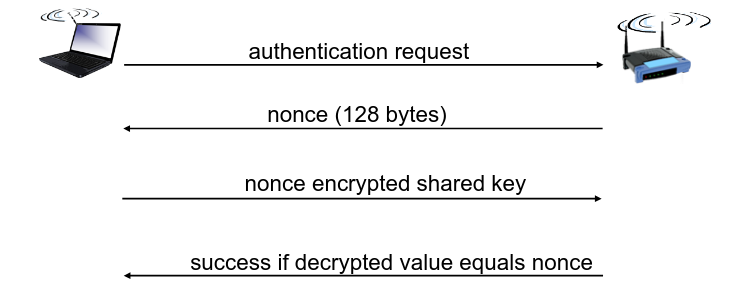
\includegraphics[width=0.7\textwidth]{img/wep.png}
\end{figure}
\paragraph{802.11i} Migliorata la sicurezza attraverso più forme di criptazioni migliori, key distribution, authentication server separato da authentication server.
\subsection{Operational security: firewalls and IDS}
\subsubsection{Firewall}
Isola una rete locale da Internet, accetta solo certi pacchetti che possono entrare mentre altri li blocca
    \begin{figure}[H]
    \centering
    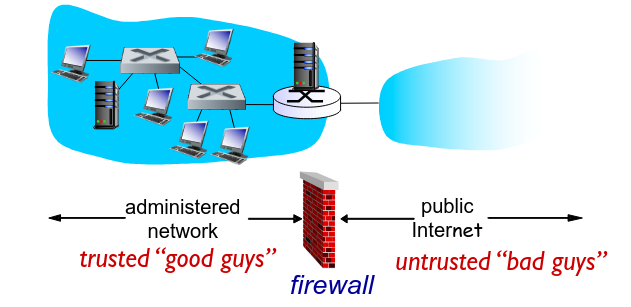
\includegraphics[width=0.7\textwidth]{img/firewall.png}
\end{figure}
I router filtrano pacchetto per pacchetto per fare il forward/drop.\\
\paragraph{Access Control Lists} Tabella di regola top-bottom per i pacchetti.
    \begin{figure}[H]
    \centering
    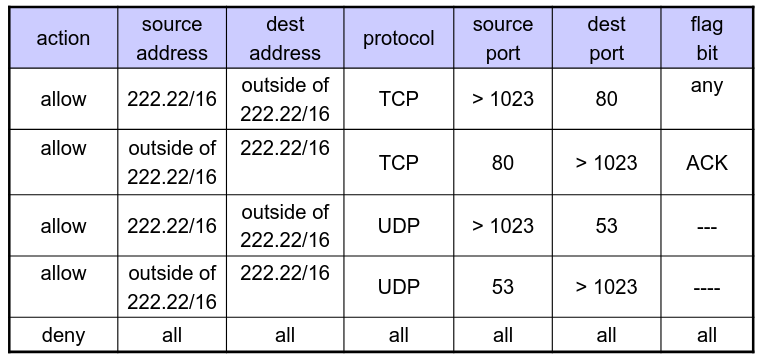
\includegraphics[width=0.7\textwidth]{img/acl.png}
\end{figure}
\begin{itemize}
  \item Stateless packet filter: guarda ogni pacchetto singolarmente
  \item Stateful packet filter: tiene traccia delle connessioni
      \begin{figure}[H]
    \centering
    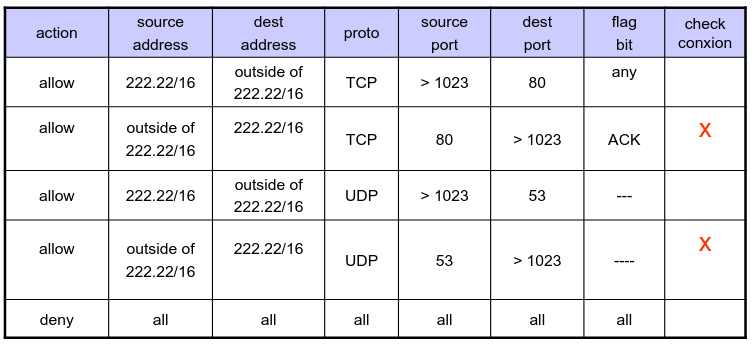
\includegraphics[width=0.7\textwidth]{img/statefull.png}
\end{figure}
\end{itemize}
\paragraph{Application gateways} Analizza il traffico capendo il protocollo applicativo (HTTP, FTP, SMTP, ecc.), per fare filtraggio avanzato. Un Application Gateway non inoltra semplicemente i pacchetti, ma analizza url, bloccare certe richieste, leggere header e cookies, ecc.
\subsubsection{IDS}
Intrusion detection system attraverso deep packet inspection e examine correlation su molteplici pacchetti.
      \begin{figure}[H]
    \centering
    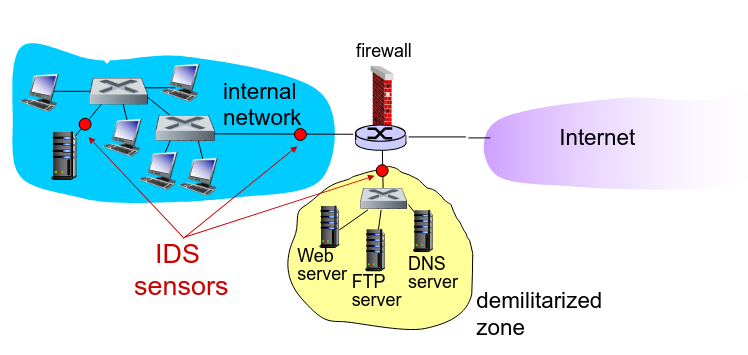
\includegraphics[width=0.7\textwidth]{img/ids.png}
\end{figure}
\section{Data Plane}
\subsection{Network layer}
Il network layer si occupa del segmento dal sender al receiver.
\begin{itemize}
  \item \textbf{Forwarding}: processo locale con cui un router inoltra ogni pacchetto dall’ingresso all’uscita corretta usando la tabella di inoltro.
  \item \textbf{Routing}: processo globale che determina i percorsi nella rete e costruisce le tabelle usate dai router.
\end{itemize}
\subsubsection{Data plane}
Funzione locale di ogni router che inoltra i datagrammi dall’ingresso all’uscita corretta (forwarding).
      \begin{figure}[H]
    \centering
    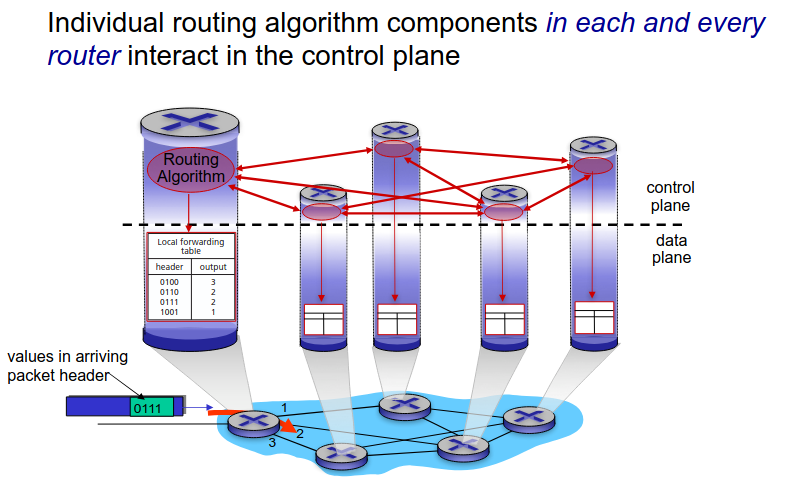
\includegraphics[width=0.7\textwidth]{img/prerouter.png}
\end{figure}
\subsubsection{Control plane}
Logica globale della rete che decide i percorsi dei datagrammi tra sorgente e destinazione (routing, via algoritmi tradizionali o SDN).
      \begin{figure}[H]
    \centering
    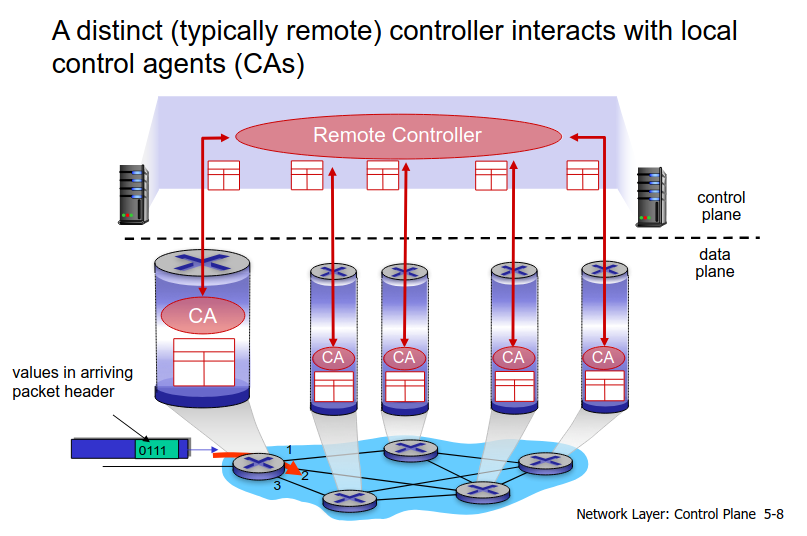
\includegraphics[width=0.7\textwidth]{img/log.png}
\end{figure}
\subsection{Come e' fatto un router}
Visione ad alto livello della architettura di un router
      \begin{figure}[H]
    \centering
    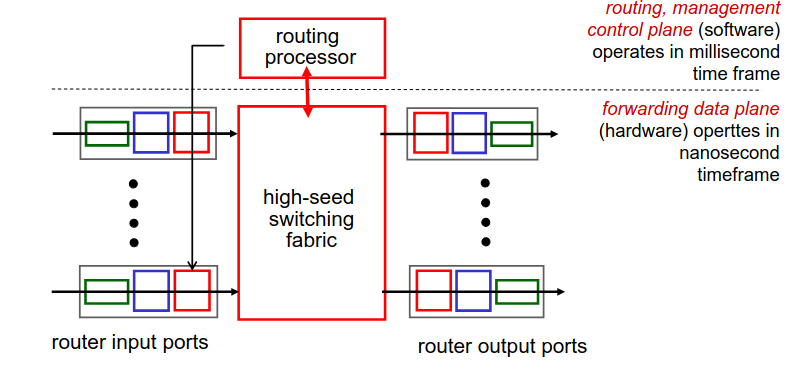
\includegraphics[width=0.7\textwidth]{img/router.png}
\end{figure}
\subsubsection{Input}
In particolare gli input sono
      \begin{figure}[H]
    \centering
    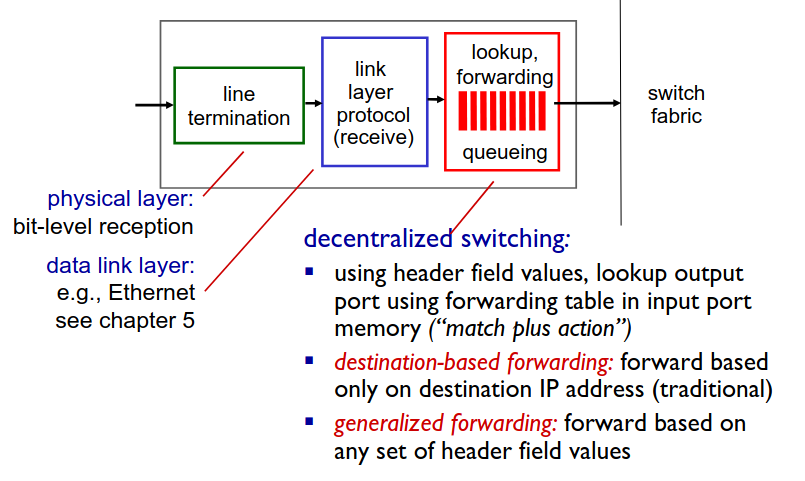
\includegraphics[width=0.7\textwidth]{img/input.png}
\end{figure}
\subsubsection*{Switching fabrics}
Trasferire un pacchetto dal input buffer ad un output buffer
      \begin{figure}[H]
    \centering
    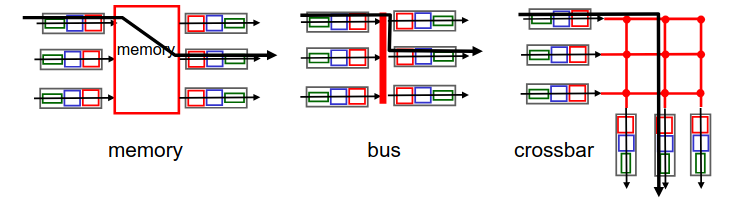
\includegraphics[width=0.7\textwidth]{img/fabrics.png}
\end{figure}
\subsubsection*{Switching via memory}
I pacchetti vengono copiati nella memoria (limitato da CPU e memory speed)
      \begin{figure}[H]
    \centering
    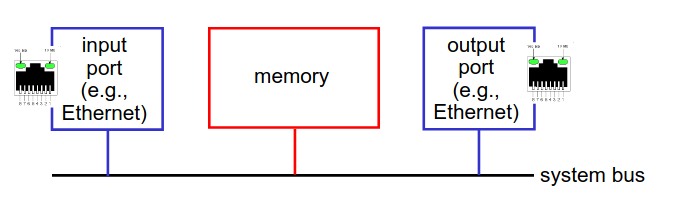
\includegraphics[width=0.7\textwidth]{img/memory.png}
\end{figure}
\subsubsection*{Switching via a bus}
Pacchetti da input memory al output memory via un bus condiviso.
      \begin{figure}[H]
    \centering
    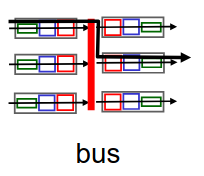
\includegraphics[width=0.3\textwidth]{img/bus.png}
\end{figure}
\subsubsection*{Switching via interconnection network}
Un crossbar è una rete interna al router che collega direttamente ogni porta di ingresso con ogni porta di uscita. (matrice, condivisione dei pacchetti in parallelo)
      \begin{figure}[H]
    \centering
    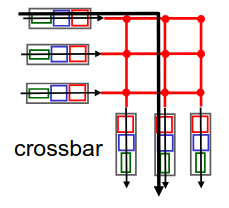
\includegraphics[width=0.3\textwidth]{img/crossbar.png}
\end{figure}
\subsubsection*{Input port queuing}
Head-of-the-Line (HOL) blocking: è quando il pacchetto in testa alla coda blocca tutti gli altri dietro, anche se potrebbero essere inoltrati verso uscite libere.
      \begin{figure}[H]
    \centering
    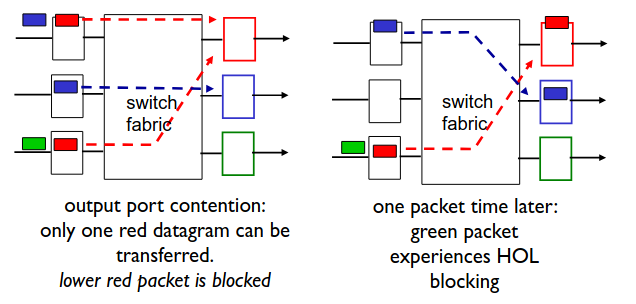
\includegraphics[width=0.5\textwidth]{img/coda.png}
\end{figure}
\subsubsection{Output}
      \begin{figure}[H]
    \centering
    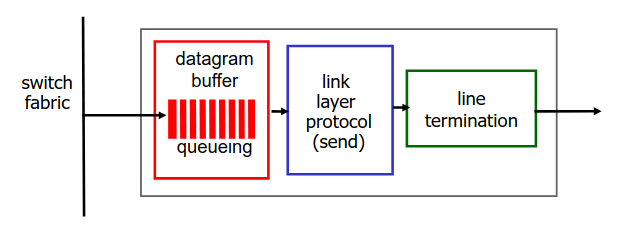
\includegraphics[width=0.5\textwidth]{img/output.png}
\end{figure}
\begin{itemize}
  \item \textbf{Buffering} (packets possono essere persi per colpa della congestione se non abbiamo un buffer)\\
  Possiamo fare buffering quando il \textit{arrival rate} supera la \textit{line speed} dello switch. Questo puo' portare loss per colpa del delay e in caso di buffer overflow.\\
  \vspace{5px}\textbf{Quanto buffer?} RFC 3439 dice: "$RTT \times C$" (con $C$ come link capacity). Es. 10Gpbs link $\Rightarrow$ 2.5Gbit buffer.\\
  O se no possiamo fare generalmente 
  \begin{align*}
    \text{buffer} = \frac{RTT \times C}{\sqrt{N}}
  \end{align*}
  \item \textbf{Scheduling} (next packet to send on link; priorita' per ottimizzare le performance)\\
  Quale meccanismo di scheduling scegliamo?
  \begin{itemize}
    \item \textbf{FIFO}
    \item \textbf{Discard policy}
    \begin{itemize}
      \item \texttt{Tail drop}
      \item \texttt{Priority}: send highest priority queued packet, supporta multiple classes, with different priorities
            \begin{figure}[H]
    \centering
    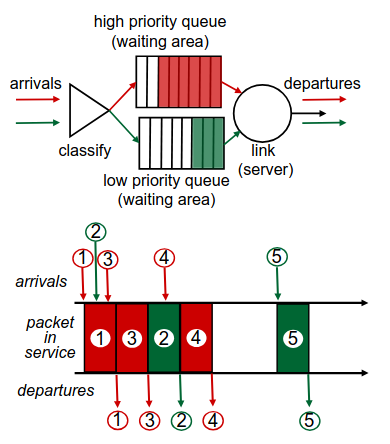
\includegraphics[width=0.5\textwidth]{img/priority.png}
\end{figure}
      \item \texttt{Random}
    \end{itemize}
    \item \textbf{Round Robin}: cyclically scan class queues, sending one complete packet from each class
                \begin{figure}[H]
    \centering
    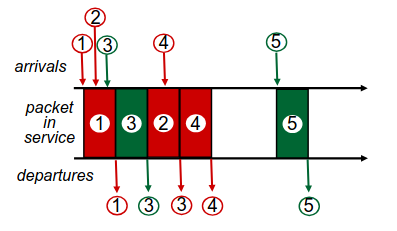
\includegraphics[width=0.5\textwidth]{img/rr.png}
\end{figure}
  \item \textbf{Weighted Fair Queuing} (WFQ): E' una generilizzazione del R.R., each class gets weighted amount of service in each cycle
                \begin{figure}[H]
    \centering
    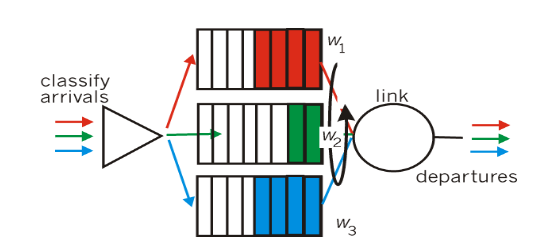
\includegraphics[width=0.5\textwidth]{img/wfq.png}
\end{figure}  
\end{itemize}
\end{itemize}
\subsection{Internet Protocol}
\subsubsection{Datagram format}
                \begin{figure}[H]
    \centering
    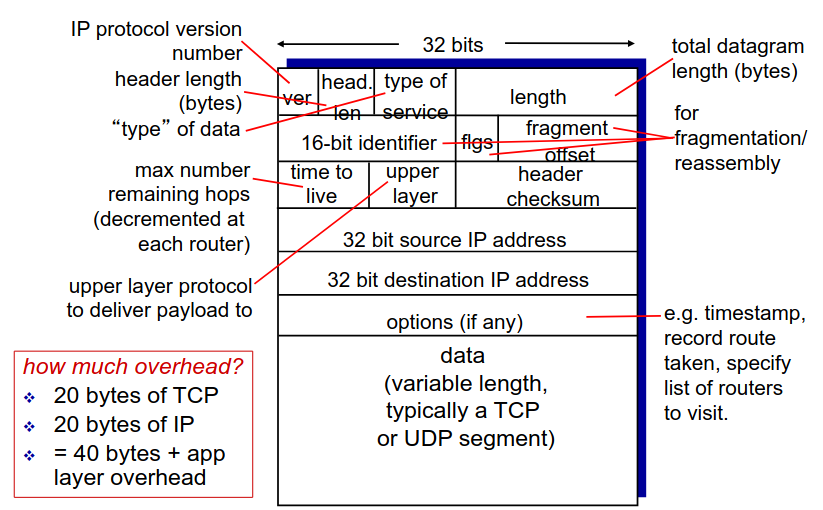
\includegraphics[width=0.8\textwidth]{img/df.png}
\end{figure}  
\subsubsection{Fragmentation}
\begin{itemize}
  \item network links have MTU
(max.transfer size) -
largest possible link-level
frame
  \item large IP datagram divided
(“fragmented”) within net
  \begin{itemize}
    \item one datagram becomes
several datagrams
    \item “reassembled” only at
final destination
    \item IP header bits used to
identify, order related
fragments
  \end{itemize}
\end{itemize}
                \begin{figure}[H]
    \centering
    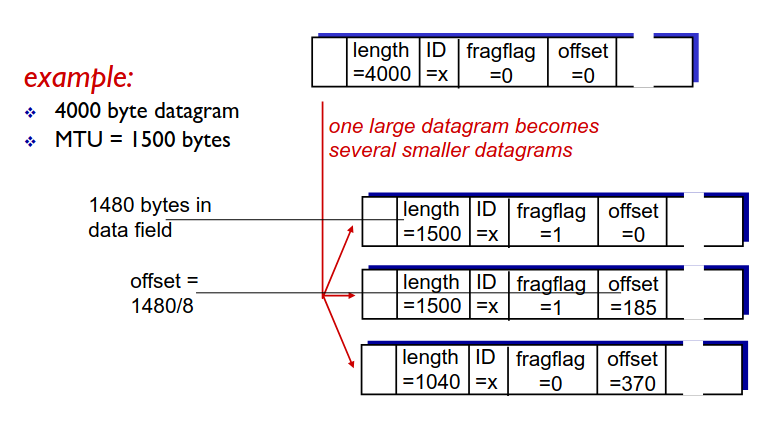
\includegraphics[width=0.8\textwidth]{img/mtu.png}
\end{figure}  
\subsubsection{IPv4 addressing}
\begin{itemize}
  \item IP address: 32 bit per host, router, interface
  \item Interface: connection
between host/router and
physical link
\end{itemize}
\paragraph{Subnets} Device interfaces with
same subnet part of IP
address. \\ 
Can physically reach
each other without
intervening router 
                \begin{figure}[H]
    \centering
    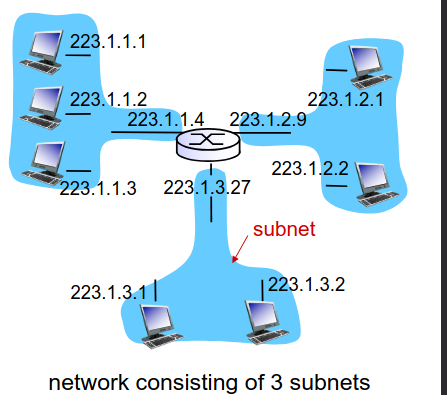
\includegraphics[width=0.4\textwidth]{img/subnet.png}
\end{figure} 
To determine the
subnets, detach each
interface from its host
or router, creating
islands of isolated
networks.\\
Each isolated network
is called a subnet.\\
\vspace{5px}\\
\paragraph{IP addressing: CIDR}
\begin{center}
  CIDR: Classless InterDomain Routing
\end{center}
\begin{itemize}
  \item Subnet portion of address of arbitrary length
  \item Address format: \texttt{a.b.c.d/x}, where \texttt{x} is \#bits in
subnet portion of address
                \begin{figure}[H]
    \centering
    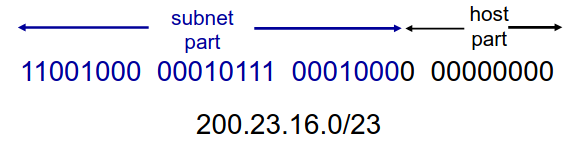
\includegraphics[width=0.4\textwidth]{img/cidr.png}
\end{figure} 
\end{itemize}
\paragraph{IP addresses: how to get one?}
\begin{itemize}
  \item \textbf{Static} (hard coded in OS)
  \item \textbf{DHCP}: Dynamic Host Configuration Protocol: dynamically get address from as server
  \begin{itemize}
    \item host broadcasts “DHCP discover” msg [optional]
    \item DHCP server responds with “DHCP offer” msg [optional]
    \item host requests IP address: “DHCP request” msg
    \item DHCP server sends address: “DHCP ack” msg
  \end{itemize}
                  \begin{figure}[H]
    \centering
    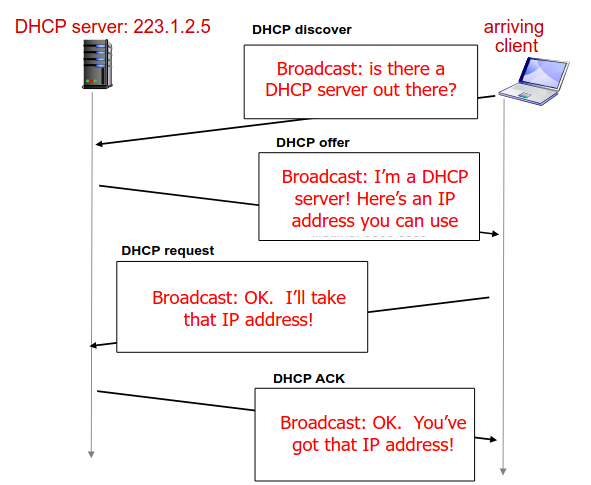
\includegraphics[width=0.6\textwidth]{img/dhcp.png}
\end{figure} 
DHCP can return more than just allocated IP
address on subnet:
\begin{itemize}
  \item address of first-hop router for client
  \item name and IP address of DNS sever
  \item network mask
\end{itemize}
\end{itemize}
\paragraph{How does an ISP get block of addresses?}
\begin{center}
  ICANN: Internet Corporation for Assigned
\end{center}
\begin{itemize}
  \item allocates addresses
  \item manages DNS
  \item assigns domain names, resolves disputes
\end{itemize}
\subsubsection{Network address translation}
                  \begin{figure}[H]
    \centering
    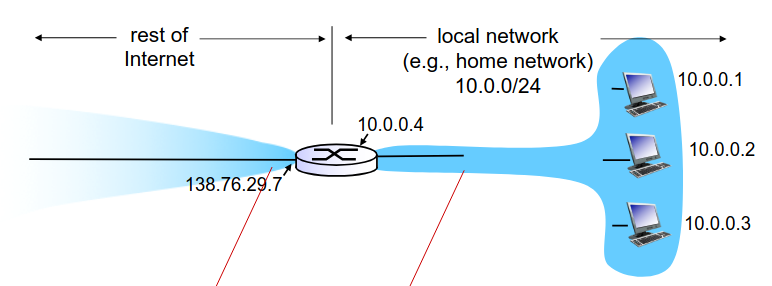
\includegraphics[width=0.7\textwidth]{img/nat.png}
\end{figure} 
\textbf{Motivation}: local network uses just one IP address as far
as outside world is concerned.\\
\texttt{NAT router must}:
\begin{itemize}
  \item \textbf{outgoing datagrams: replace} (source IP address, port \#) of
every outgoing datagram to (NAT IP address, new port \#)
  \item \textbf{remember (in NAT translation table)} every (source IP address,
port \#) to (NAT IP address, new port \#) translation pair
  \item incoming datagrams: replace (NAT IP address, new port \#) in
dest fields of every incoming datagram with corresponding
(source IP address, port \#) stored in NAT table
\end{itemize}
                  \begin{figure}[H]
    \centering
    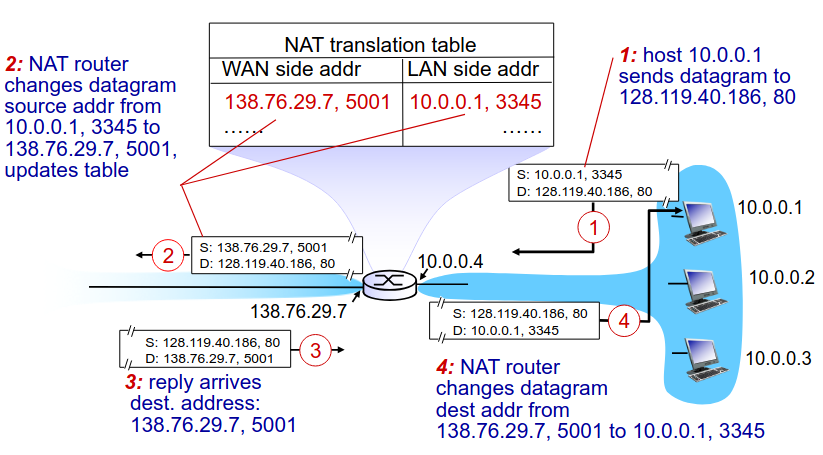
\includegraphics[width=0.7\textwidth]{img/nat2.png}
\end{figure} 
\subsubsection{IPv6}
\textbf{Initial motivation:} 32-bit address space soon to be
completely allocated. \\
\textbf{Extra}: header format helps speed processing/forwarding and header changes to facilitate QoS.
\paragraph{IPv6 datagram format}
\begin{itemize}
  \item 40byte fixed header
  \item no fragmentation allowed
\end{itemize}
                  \begin{figure}[H]
    \centering
    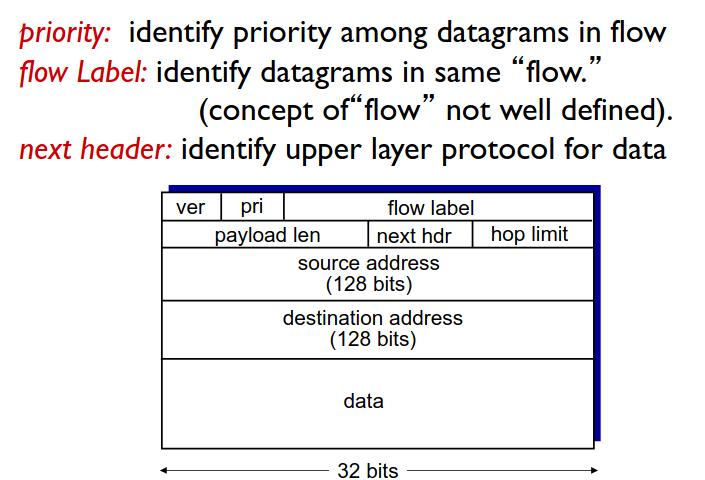
\includegraphics[width=0.7\textwidth]{img/df6.png}
\end{figure} 
\paragraph{How will network operate with mixed IPv4 and
IPv6 routers?} \textbf{Tunneling!} IPv6 datagram carried as payload in IPv4
datagram among IPv4 routers
                  \begin{figure}[H]
    \centering
    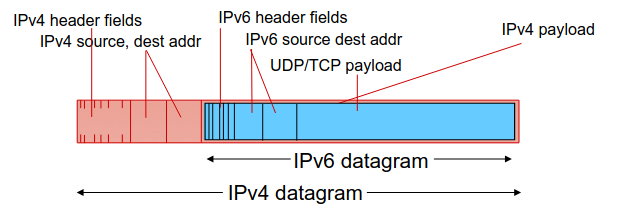
\includegraphics[width=0.7\textwidth]{img/tunnelling1.png}
\end{figure} 
                  \begin{figure}[H]
    \centering
    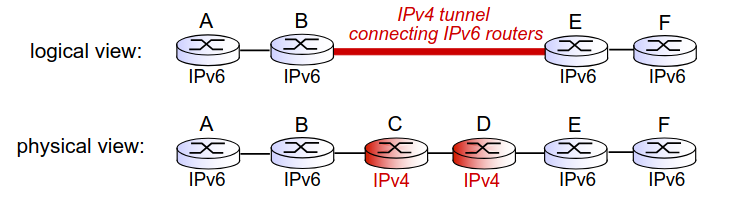
\includegraphics[width=0.7\textwidth]{img/tunneling2.png}
\end{figure} 
\subsection{Generalized Forward and SDN}
Each router contains a flow table that is computed and
distributed by a logically centralized routing controller
                  \begin{figure}[H]
    \centering
    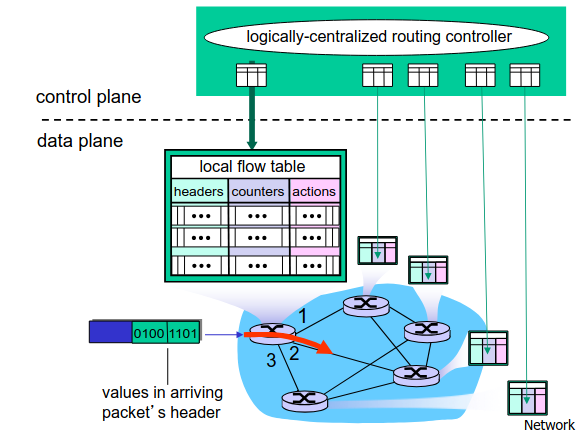
\includegraphics[width=0.7\textwidth]{img/sdn.png}
\end{figure} 
\subsubsection{OpenFlow data plane abstraction}
\begin{itemize}
  \item flow: defined by header fields
  \item generalized forwarding: simple packet-handling rules
  \begin{itemize}
    \item Pattern: match values in packet header fields
    \item Actions: for matched packet: drop, forward, modify, matched
packet or send matched packet to controller
    \item Priority: disambiguate overlapping patterns
    \item Counters: \#bytes and \#packets
  \end{itemize}
\end{itemize}
\section{Control Plane}
\end{document}

